\chapter{TASK\_1.}

\textbf{Цель работы:}

\begin{itemize} 
	\item Создать сервер;
	\item Работа с POST запросами;
	\item Работа с GET запросами;
	\item Работа с CSS.
\end{itemize}

\textbf{Задание 1}

Создать сервер. Сервер должен выдавать страницу с тремя текстовыми полями и кнопкой. В поля ввода вбивается информация о почте, фамилии и номере телефона человека. При нажатии на кнопку "Отправить" введённая информация должна отправляться с помощью POST запроса на сервер и добавляться к концу файла (в файле накапливается информация). При этом на стороне сервера должна происходить проверка: являются ли почта и телефон уникальными. Если они уникальны, то идёт добавление информации в файл. В противном случае добавление не происходит. При отправке ответа с сервера клиенту должно приходить сообщение с информацией о результате добавления (добавилось или не добавилось). Результат операции должен отображаться на странице.

\textbf{Задание 2}

Добавить серверу возможность отправлять клиенту ещё одну страницу. На данной странице должно быть поле ввода и кнопка. В поле ввода вводится почта человека. При нажатии на кнопку "Отправить" на сервер отправляется GET запрос. Сервер в ответ на GET запрос должен отправить информацию о человеке с данной почтой в формате JSON или сообщение об отсутствии человека с данной почтой.

\textbf{Задание 3}

Оформить внешний вид созданных страниц с помощью CSS. Информация со стилями CSS для каждой страницы должна храниться в отдельном файле. Стили CSS должны быть подключены к страницам.

\begin{lstlisting}[caption=Код программы. TASK\_1. Код программы]
"use strict";

// импортируем необходимые библиотеки
const express = require("express");
const fs = require("fs");

const ENCODING = "utf-8"
const fileName = "data/user.json";

function main() {
	// Запускаем сервер.
	const app = express();
	const port = 5000;
	app.listen(port);
	console.log(`Server on port ${port}`);

	// Отправка статических файлов.
	const way = __dirname + "/static";
	app.use(express.static(way));

	// Получение информации.
	// Это GET запрос он получает 
	// В url некоторые аргументы.
	// Не имеет тела.
	app.get("/find", function (request, response) {
		const mail = request.query.mail;
		let res = "Нет информации.";

		// Открываем файл и парсим.
		const objInfo = fs.readFileSync(fileName, "utf-8");
		const infoJson = JSON.parse(objInfo);

		// Проверяем наличие.
		for (let i in infoJson) {
			if (mail == infoJson[i].mail) {
				res = infoJson[i];
				break;
			}
		}

		response.end(JSON.stringify({
			result: JSON.stringify(res)
		}));
	});

	app.get("/get_info", (_request, response) => {
		const fileContent = fs.readFileSync("static/" + "get_info.html", ENCODING);
		response.end(fileContent);
	});


	// body
	// Тут получаем данные тела.
	function loadBody(request, callback) {
		let body = [];
		request.on('data', (chunk) => {
			body.push(chunk);
		}).on('end', () => {
			body = Buffer.concat(body).toString();
			callback(body);
		});
	}

	// it is post
	app.post("/save/info", function (request, response) {
		loadBody(request, function (body) {
			// Файл, содержащий бд пользователей.

			// Получаем данные.
			const obj = JSON.parse(body);
			const mail = obj["mail"];
			const surname = obj["surname"];
			const phone_number = obj["phone_number"];

			// Открываем файл и парсим.
			const objInfo = fs.readFileSync(fileName, "utf-8");
			const infoJson = JSON.parse(objInfo);

			// true - нужно добавить.
			// false - уже имеется юзер.
			let flag = true;
			// Текст, который увидит пользователь.
			let text = "";

			// Проверяем уникальность.
			for (let i in infoJson) {
				if (mail == infoJson[i].mail) {
					flag = false;
					text = "Данная почта уже имеется в системе!"
					break;
				}
				if (phone_number == infoJson[i].phone_number) {
					flag = false;
					text = "Данный номер уже имеется в системе!"
					break;
				}
			}

			// Если уникальный, добавляем в нашу БД.
			// И меняем сообщение на то, что инфа добавлена.
			if (flag) {
				infoJson.push({ mail, surname, phone_number })
				fs.writeFileSync(fileName, JSON.stringify(infoJson, null, 4));
				text = "Информация успешно добавлена!"
			}

			// Ответ запроса.
			response.end(JSON.stringify({
				result: text
			}));
		});
	});
}


main();
\end{lstlisting}

\begin{lstlisting}[caption=Код программы. TASK\_1. Дополнительный скрипт]
	"use strict";

// onload - функция, которая вызывается когда собрался HTML.
// window - это глобальной объект.
window.onload = function () {
	// Получаем (ссылку) на поля.
	const field_find_mail = document.getElementById("field-get-info");

	// Получаем кнопку, при нажатии на которую должна выдаваться информация.
	const btn_get_info = document.getElementById("get-info-btn");

	// ajax get
	function ajaxGet(urlString, callback) {
		let r = new XMLHttpRequest();
		r.open("GET", urlString, true);
		r.setRequestHeader("Content-Type", "text/plain;charset=UTF-8");
		r.send(null);
		r.onload = function () {
			callback(r.response);
		};
	};

	btn_get_info.onclick = function () {
		const find_mail = field_find_mail.value;

		const url = `/find?mail=${find_mail}`;

		ajaxGet(url, function (stringAnswer) {
			const objectAnswer = JSON.parse(stringAnswer);
			const result = objectAnswer.result;
			alert(result);
		});
	}
};
\end{lstlisting}

\begin{lstlisting}[caption=Код программы. TASK\_1. Дополнительный скрипт]
	"use strict";

	// onload - функция, которая вызывается когда собрался HTML.
	// window - это глобальной объект.
	window.onload = function () {
		// Получаем (ссылку) на поля.
		const field_mail = document.getElementById("field-mail");
		const field_surname = document.getElementById("field-surname");
		const field_phone_number = document.getElementById("field-phone_number");
	
		// Получаем кнопку, при нажатии на которую должна добавляться информация.
		const btn_add_info = document.getElementById("add-info-btn");
	
		// Метка, на которой будет отображен результат добваления (Добавилось/Не добавилось).
		const label = document.getElementById("result-label");
	
		function ajaxPost(urlString, bodyString, callback) {
			let r = new XMLHttpRequest();
			r.open("POST", urlString, true);
			r.setRequestHeader("Content-Type", "application/json;charset=UTF-8");
			r.send(bodyString);
			r.onload = function () {
				callback(r.response);
			}
		}
	
		// Событие: нажали на кнопку.
		btn_add_info.onclick = function () {
			const mail = field_mail.value;
			const surname = field_surname.value;
			const phone_number = field_phone_number.value;
	
			// Создаем POST запрос. 
			// В тело предаем mail, surname, phone_number.
			ajaxPost("/save/info", JSON.stringify({
				mail, surname, phone_number
			}), function (answerString) {
				const answerObject = JSON.parse(answerString);
				const result = answerObject.result;
				label.innerHTML = result;
			});
		};
	};
\end{lstlisting}

\textbf{Вывод:}

\begin{itemize} 
	\item Был создан сервер;
	\item Была реализована работа с POST запросами;
	\item Была реализована работа с GET запросами;
	\item Была реализована работа с CSS.
\end{itemize}

\textbf{Пример работы:}

\begin{figure}[ht!]
	\centering{
		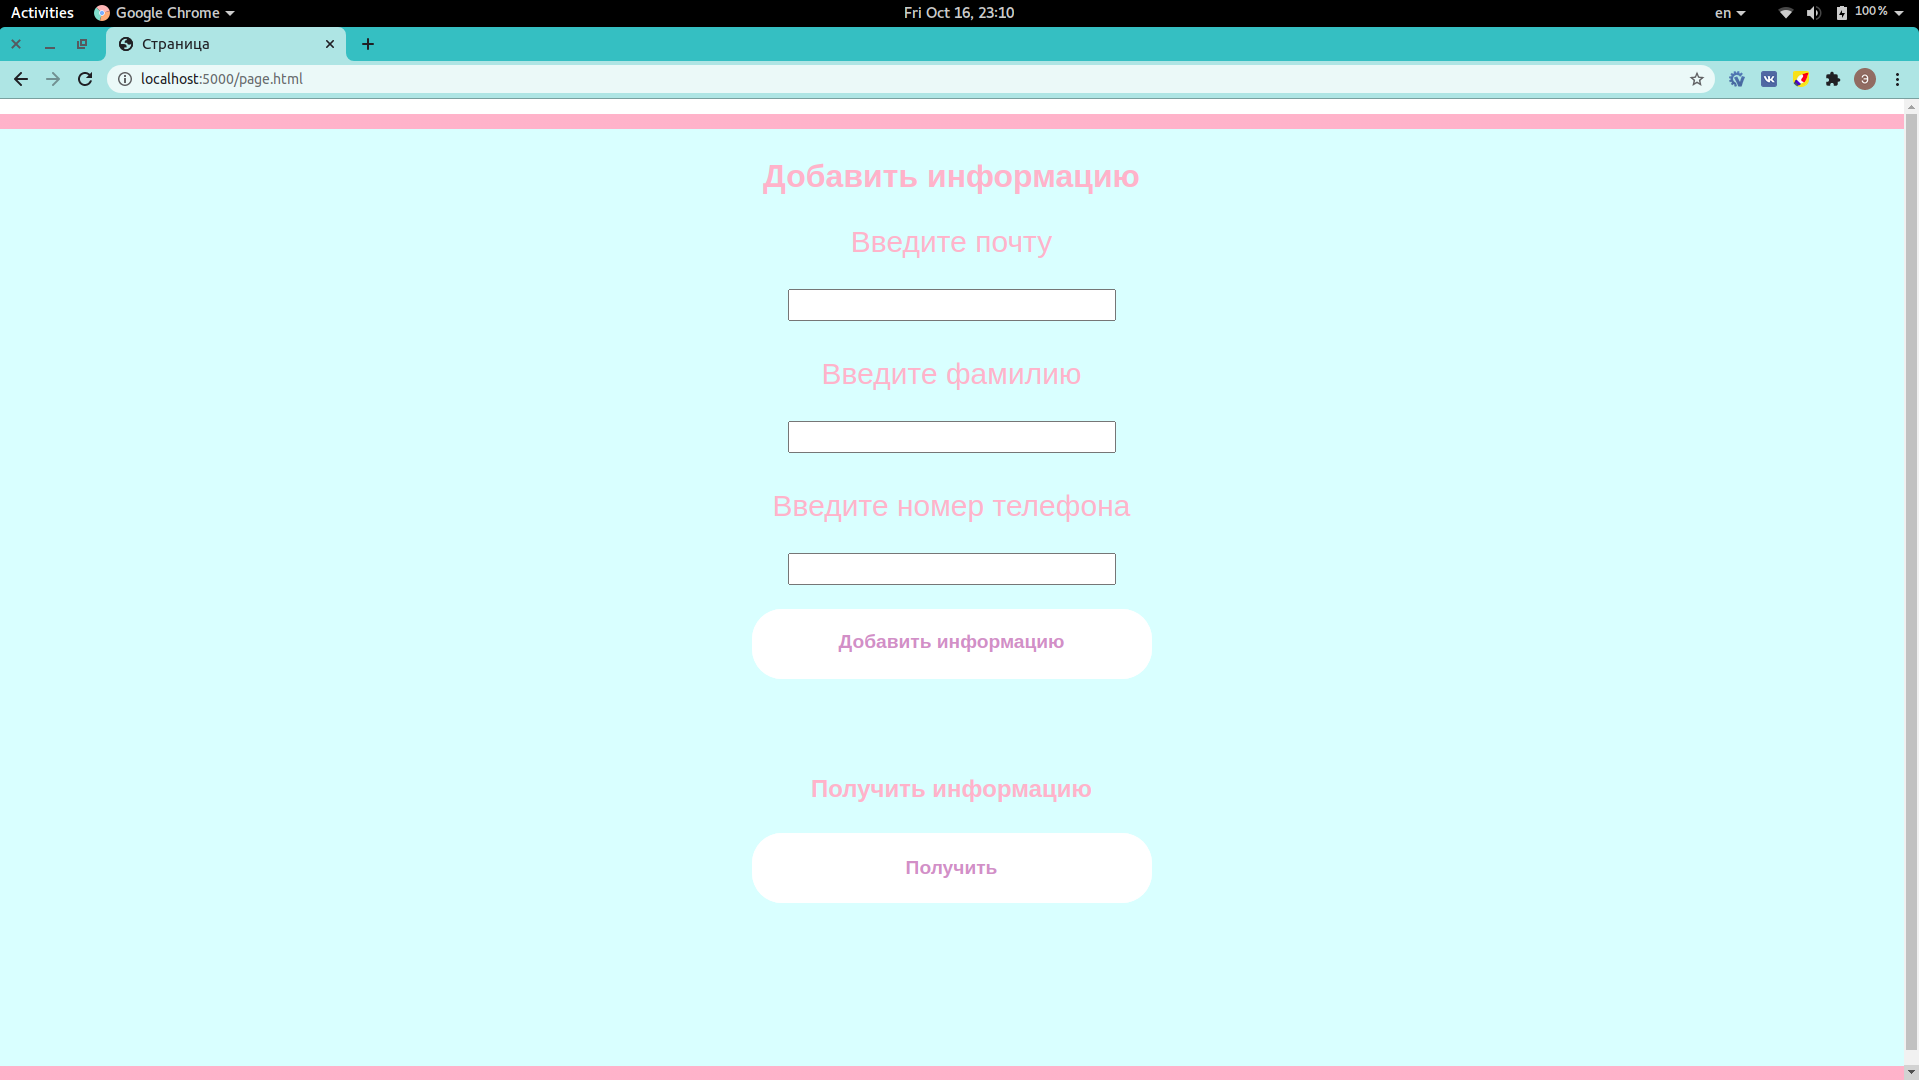
\includegraphics[width=0.9\textwidth]{img/7.png}
		\caption{Пример работы программы}}
\end{figure}


\begin{figure}[ht!]
	\centering{
		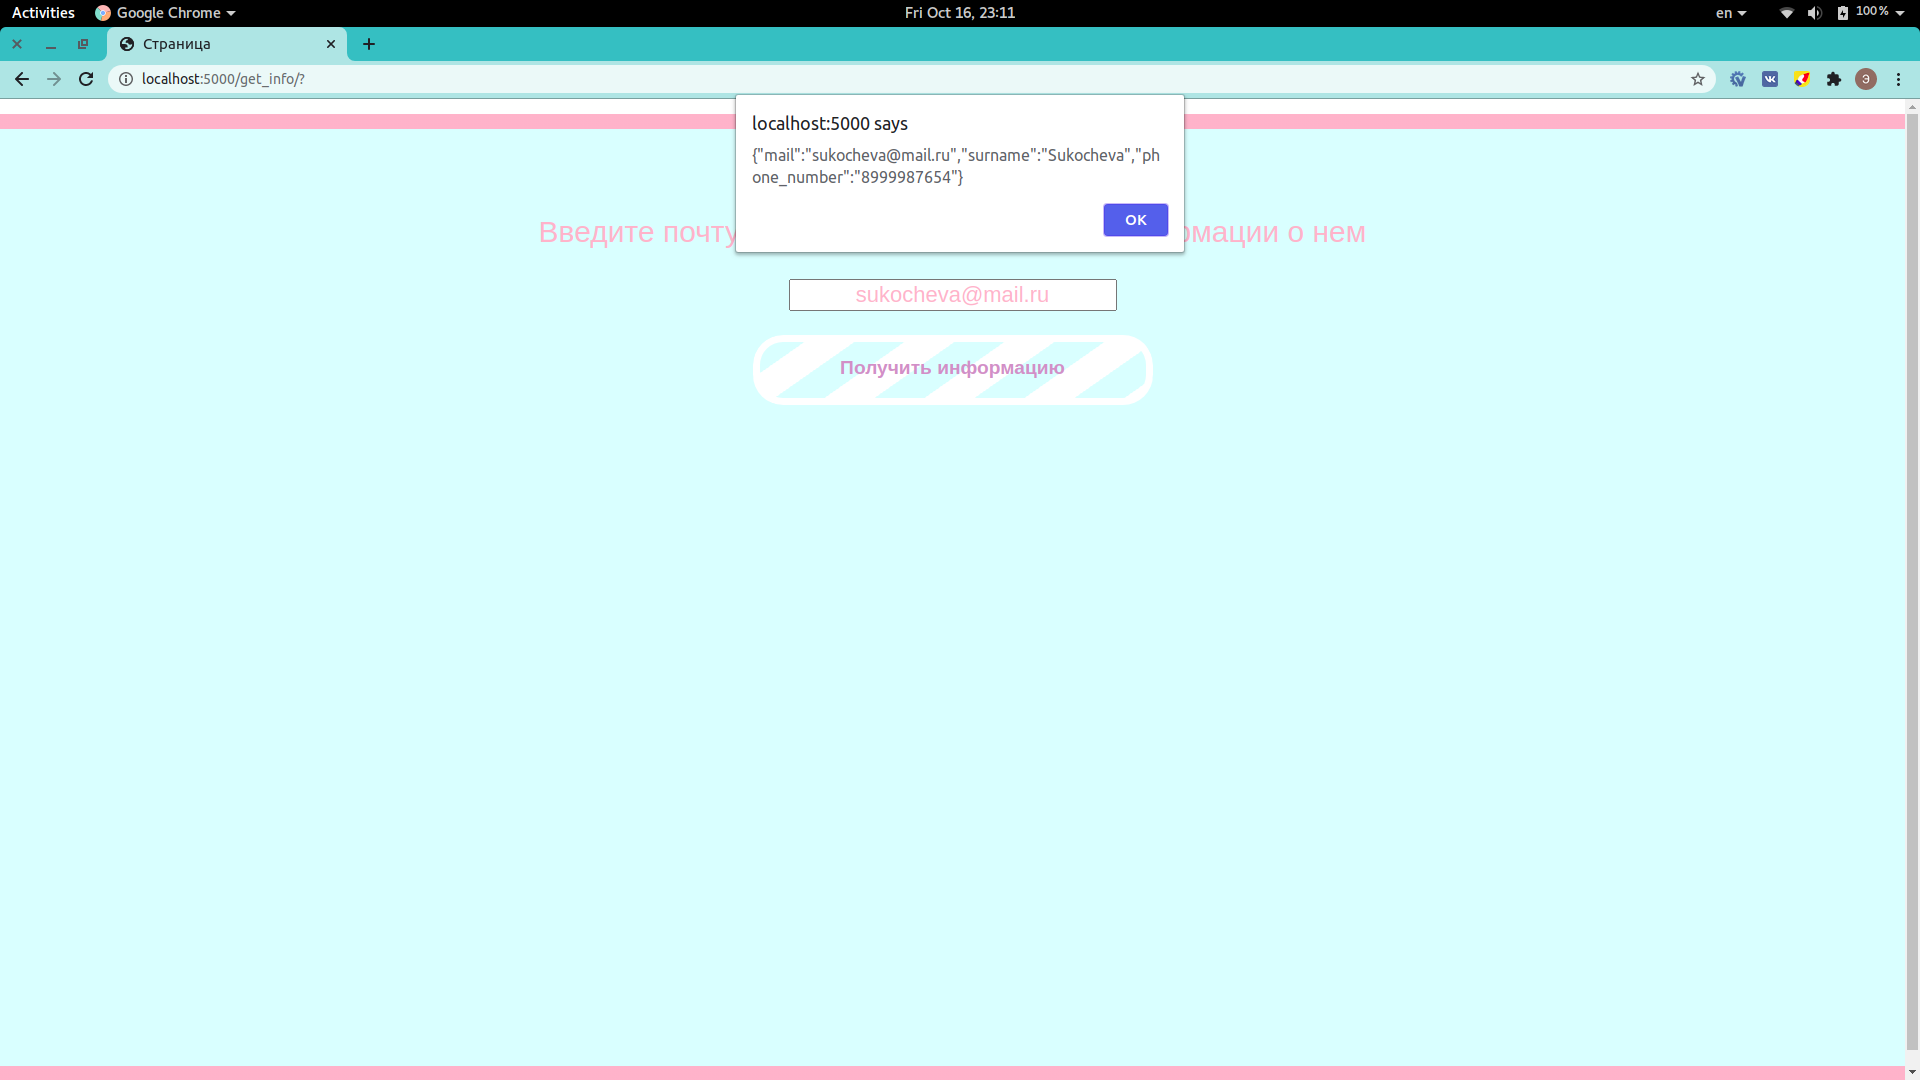
\includegraphics[width=0.9\textwidth]{img/8.png}
		\caption{Пример работы программы}}
\end{figure}

\begin{figure}[ht!]
	\centering{
		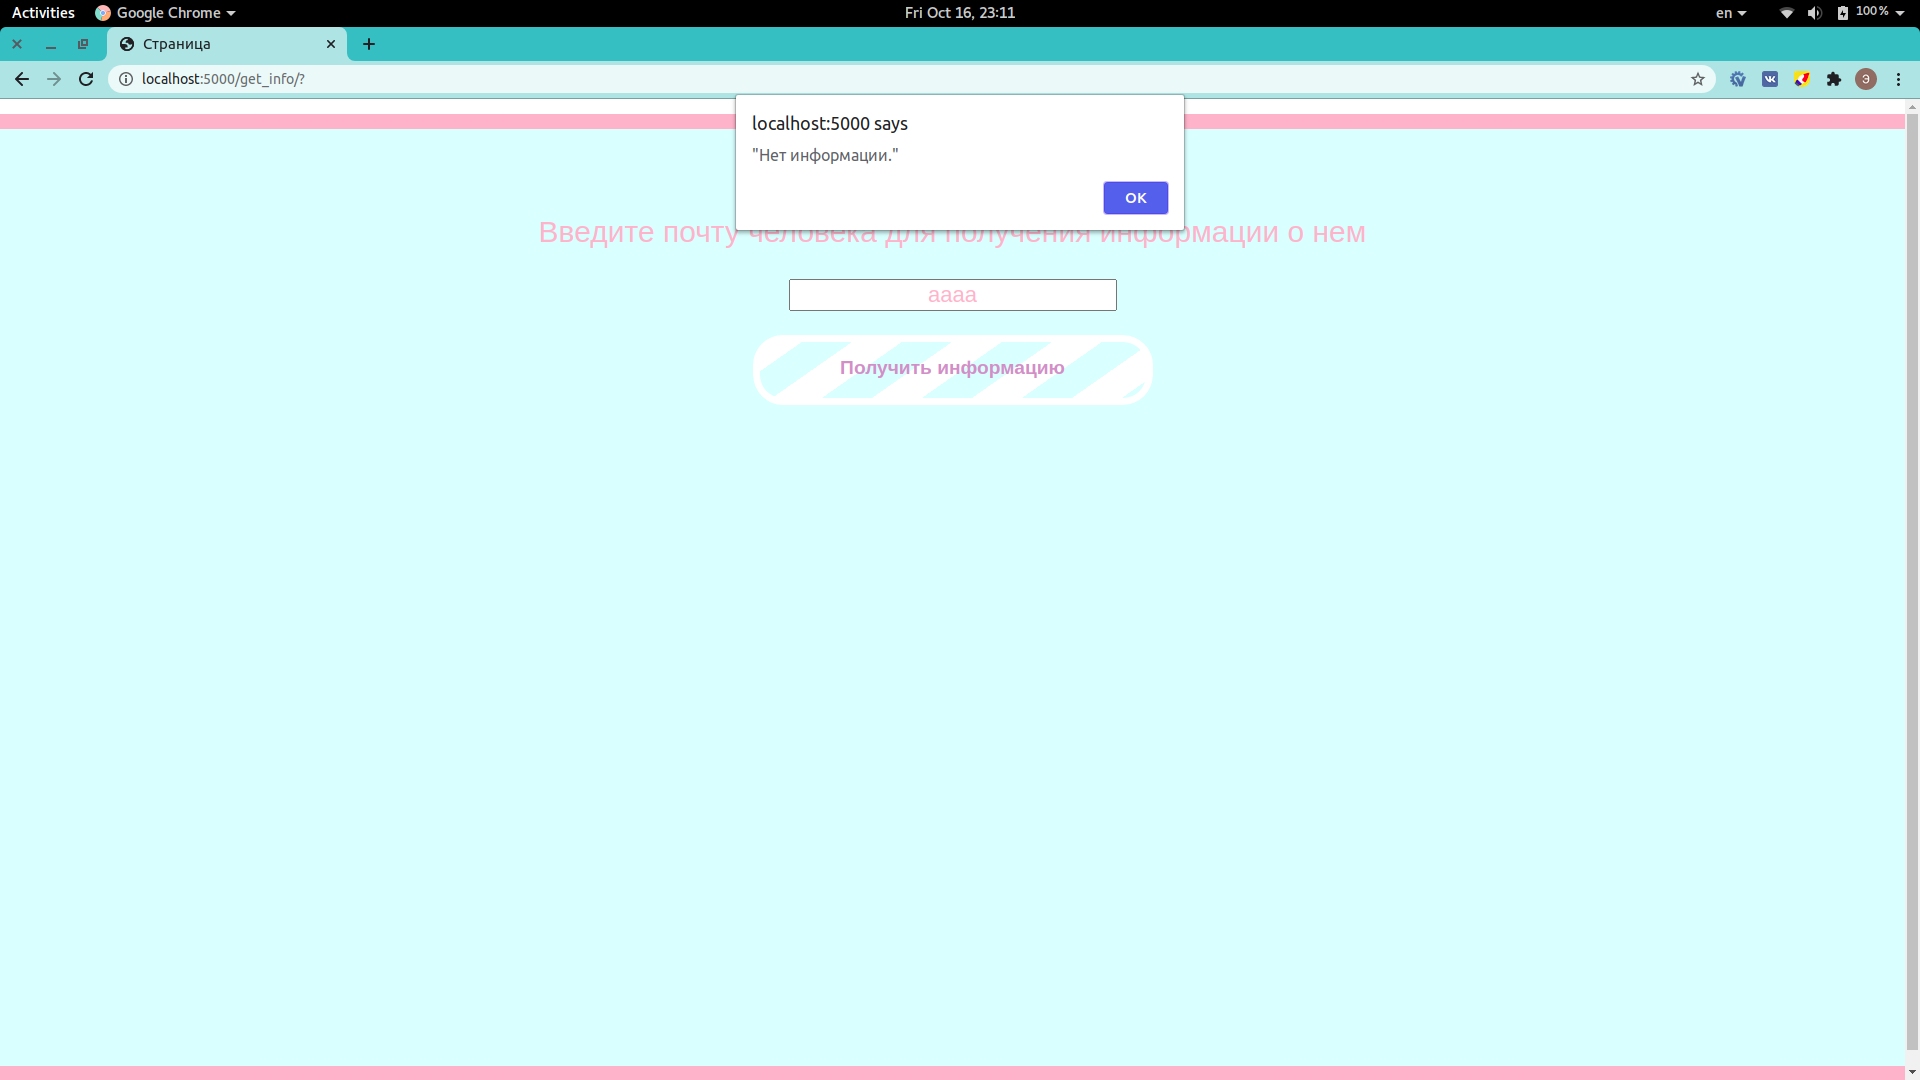
\includegraphics[width=0.9\textwidth]{img/9.png}
		\caption{Пример работы программы}}
\end{figure}

\chapter{TASK\_2.}

\textbf{Цель работы:}

\begin{itemize} 
	\item Создать сервер.
	\item Реализовать страницу с использованием шаблонизатора.
	\item Изучить и реализовать работу с cookie.
\end{itemize}

\textbf{Задание 1}

Создать сервер. В оперативной памяти на стороне сервера создать массив, в котором хранится информация о компьютерных играх (название игры, описание игры, возрастные ограничения). Создать страницу с помощью шаблонизатора. В url передаётся параметр возраст (целое число). Необходимо отображать на этой странице только те игры, у которых возрастное ограничение меньше, чем переданное в url значение.

\textbf{Задание 2}

Создать сервер. В оперативной памяти на стороне сервера создать массив, в котором хранится информация о пользователях (логин, пароль, хобби, возраст). На основе cookie реализовать авторизацию пользователей. Реализовать возможность для авторизованного пользователя просматривать информацию о себе.

\begin{lstlisting}[caption=Код программы. TASK\_2. Реализация задания 1]
	"use strict";

	// Импорт библиотек.
	const express = require("express");
	// Импорт библиотеки для работы с файлами.
	const fs = require("fs");

	function main() {
		// запускаем сервер
		const app = express();
		const port = 5000;
		app.listen(port);
		console.log(`Server on port ${port}`);
	
		// Активируем шаблонизатор.
		app.set("view engine", "hbs");
	
		// Выдаем страницу с массивом игр, у которых возрастное
		// Ограничение младше, чем то, которое передано в url.
		app.get("/page/pupils", function (request, response) {
			// Получаем возраст,введенный пользователем из url.
			let age = request.query.age;
			age = parseInt(age);
			// Если корявый url пришел, сообщаем обо этом и выходим из метода.
			if (!age) {
				response.end("Age input error!");
				return
			}
	
			// Открываем файл с играми.
			const FILE_NAME = __dirname + "/game.json";
			const contentFile = fs.readFileSync(FILE_NAME, "utf-8");
			const gamesArray = JSON.parse(contentFile);
			// Создаем результирующий массив,
			// В котором будут удовлетворяющие условию игры. 
			const resultArray = [];
	
			// Пробегаемся по всем имеющимся играм.
			for (let i = 0; i < gamesArray.length; i++) {
				// Если удовлетворяет условию 
				// Добавляем в результурующий массив.
				if (gamesArray[i].age_limit < age)
					resultArray.push(gamesArray[i])
			}
			// Создаем объект, которые подставится в шаблонизатор.
			const infoObject = {
				// Описание.
				descriptionValue: "Games list:",
				// Массив игр.
				gamesArray: resultArray
			};
	
			response.render("pageGames.hbs", infoObject);
		});
	}
	
	main()
\end{lstlisting}


\begin{lstlisting}[caption=Код программы. TASK\_2. Реализация задания 2]
	"use strict";
	
	// импортируем библиотеки
	const express = require("express");
	const cookieSession = require("cookie-session");
	const fs = require("fs");
	
	function main() {
		// запускаем сервер
		const app = express();
		const port = 5000;
		app.listen(port);
		console.log(`Server on port ${port}`);
	
		// Работа с сессией.
		app.use(cookieSession({
			name: 'session',
			keys: ['hhh', 'qqq', 'vvv'],
			maxAge: 24 * 60 * 60 * 1000 * 365
		}));
	
		// Авторизация.
		// Принимает два параметра:
		// Логин и пароль.
		app.get("/api/sign_in", function (request, response) {
			// Если пользователь уже авторизован
			// То сообщаем ему об этом.
			if (request.session.login) {
				return response.end("You are sign in.");
			}
	
			// Получаем параметры запроса.
			const login = request.query.login;
			const password = request.query.password;
	
			// Проверяем существование.
			if (!login) return response.end("Login not set");
			if (!password) return response.end("password not set");
	
	
			// Если пользователь не авторизирован и 
			// Если такой пользователь есть в 
			// Нашем массиве, то выставляем для него cookie.
			const FILE_NAME = "data.json";
			const jsonString = fs.readFileSync(FILE_NAME, "utf-8");
			const obj = JSON.parse(jsonString);
	
			for (let i = 0; i < obj.length; i++) {
				if (obj[i].login === login && obj[i].password == password) {
					request.session.login = login;
					request.session.password = password;
					return response.end("Ok!");
				}
			}
	
			response.end("Invalid Login or password.");
		});
	
		// Получить данные.
		// Если пользователь авторизирован 
		// (Т.е. есть куки), то выдаем информацию о нем.
		app.get("/api/get_info", function (request, response) {
			// Получаем cookie пользователя.
			let login = request.session.login;
			let password = request.session.password;
	
			// Контролируем существование cookie.
			if (!login) return response.end("Not exists");
			if (!password) return response.end("Not exists");
	
			// Если пользователь авторизирован (cookie существуют)
			// То выдаем информацию о нем (из файла).
			const FILE_NAME = "data.json";
			const jsonString = fs.readFileSync(FILE_NAME, "utf-8");
			const obj = JSON.parse(jsonString);
	
			for (let i = 0; i < obj.length; i++) {
				if (obj[i].login === login && obj[i].password == password) {
					let answer = "Information:\nlogin:" + obj[i].login + "\nAge:" + obj[i].age +
						"\nHobby: " + obj[i].hobby;
					return response.end(answer);
				}
			}
	
			response.end("No information!");
		});
	
		// Выход из системы.
		app.get("/api/sign_out", function (request, response) {
			// Удалить все cookie.
			request.session = null;
			response.end("You are sign out!");
		});
	}
	
	main()	
\end{lstlisting}

\textbf{Вывод:}

\begin{itemize} 
	\item Был создан сервер.
	\item Была реализована страница с использованием шаблонизатора.
	\item Была изучена и реализована работа с cookie.
\end{itemize}


\textbf{Пример работы:}

\begin{figure}[ht!]
	\centering{
		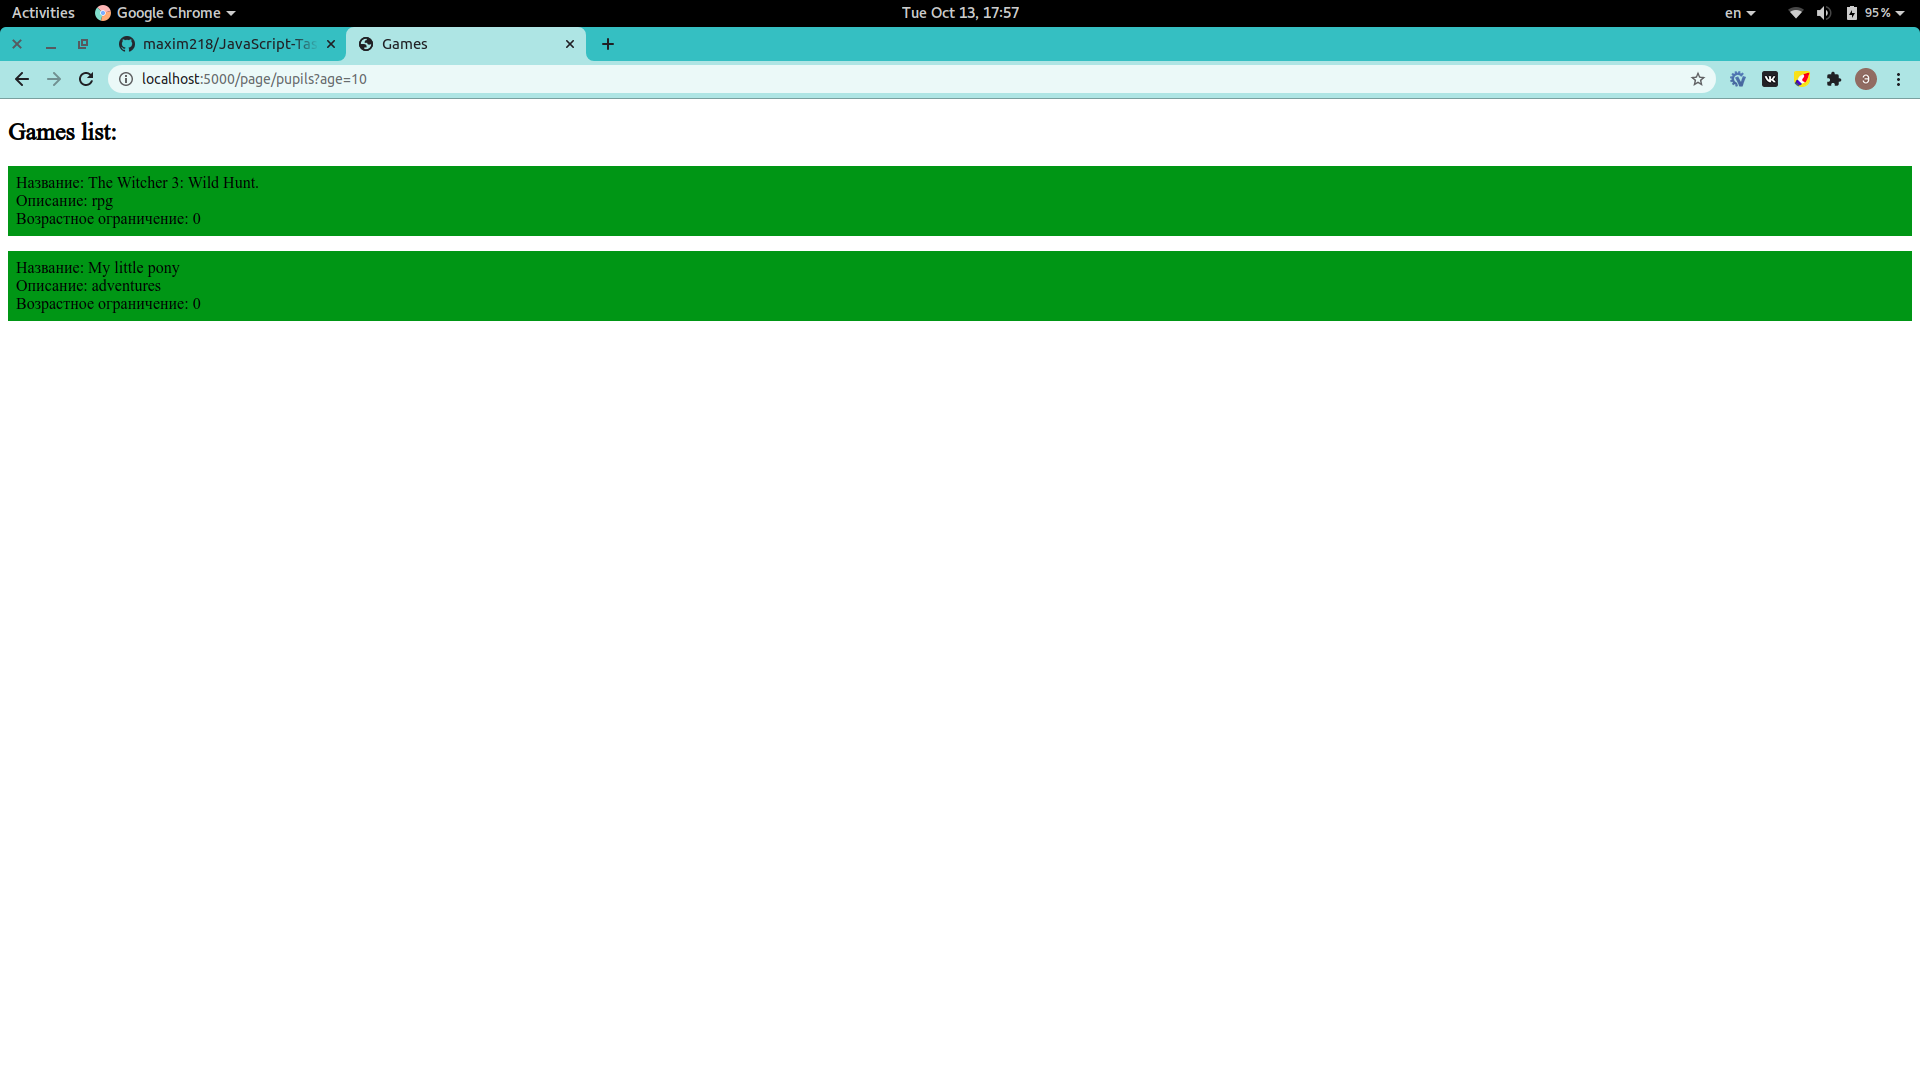
\includegraphics[width=0.9\textwidth]{img/1.png}
		\caption{Пример работы программы}}
\end{figure}

\begin{figure}[ht!]
	\centering{
		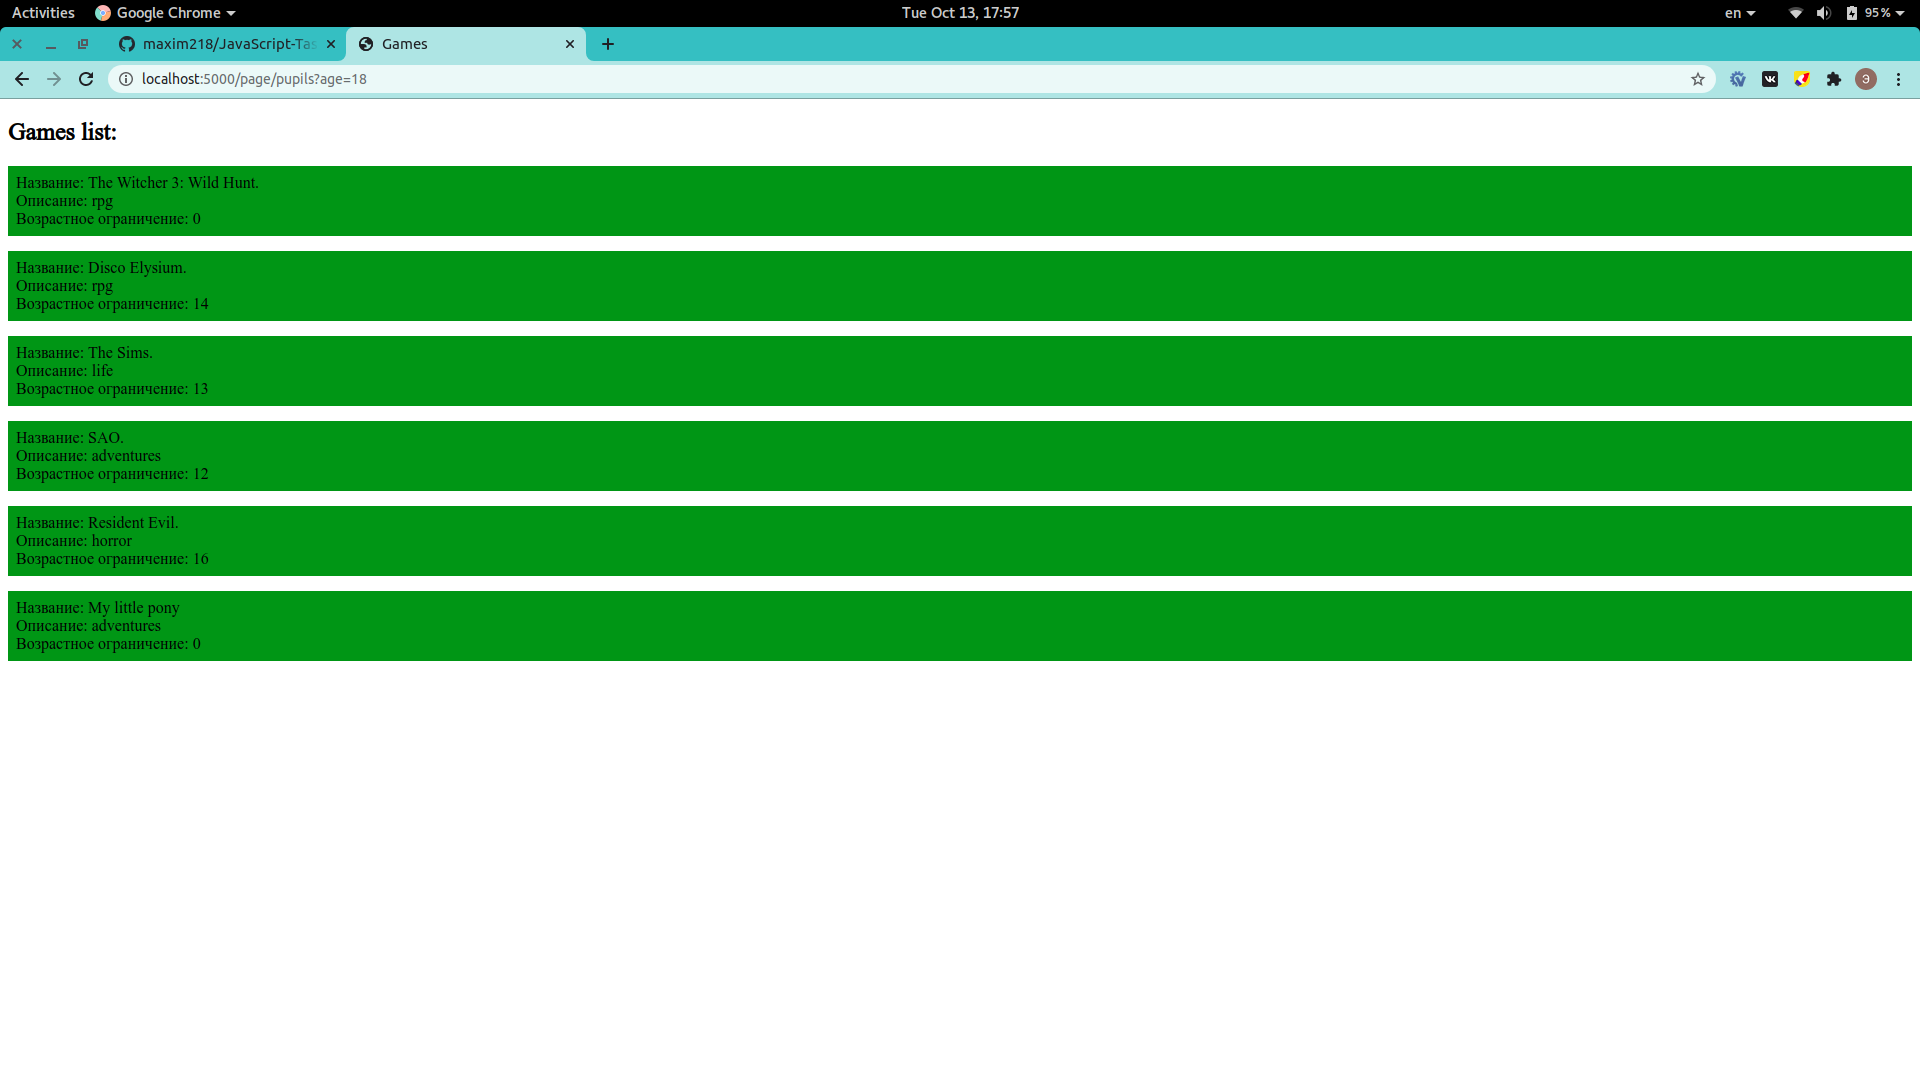
\includegraphics[width=0.9\textwidth]{img/2.png}
		\caption{Пример работы программы}}
\end{figure}

\begin{figure}[ht!]
	\centering{
		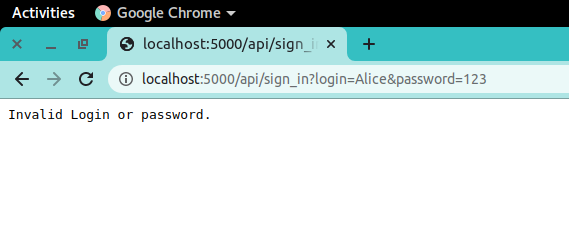
\includegraphics[width=0.9\textwidth]{img/3.png}
		\caption{Пример работы программы}}
\end{figure}

\begin{figure}[ht!]
	\centering{
		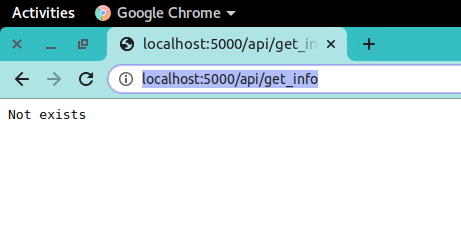
\includegraphics[width=0.9\textwidth]{img/4.png}
		\caption{Пример работы программы}}
\end{figure}

\begin{figure}[ht!]
	\centering{
		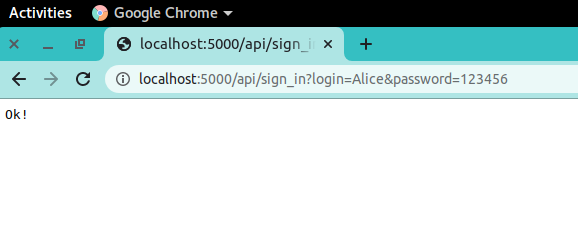
\includegraphics[width=0.9\textwidth]{img/5.png}
		\caption{Пример работы программы}}
\end{figure}

\begin{figure}[ht!]
	\centering{
		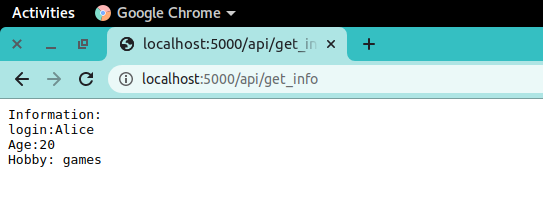
\includegraphics[width=0.9\textwidth]{img/6.png}
		\caption{Пример работы программы}}
\end{figure}
